\chapter*{Frequency response of Pioneer A-616}
A test was made to get a view of the frequency response of the Pioneer A-616 amplifier. The Pioneer A-616 amplifier is used for all measurement in this project, and therefore the frequency response is of interest. To measure the frequency response, the function from \autoref{appendix:transfer_function} is used. The test is done with and without load, to find out if the load changes the transfer function of the amplifier.

\section*{Materials and setup}
To measure the frequency response of the Pioneer A-616 amplifier, the following materials are used:
\begin{itemize}
\item RME FIREFACE UCX (Soundcard)
\begin{itemize}[noitemsep]
\item AAU-number: 108230
\item Serial number: 23811948
\end{itemize}
\item Pioneer A-616 with a gain of \SI{44}{\decibel} (amplifier)
\begin{itemize}[noitemsep]
\item AAU-number: B4-109-C-8
\item Serial number: HJ9404841S
\end{itemize}
\item MATLAB 2017b (PC - Software)
\item IRmeas_fft (software) \autoref{appendix:transfer_function}
\item SEAS 33 F-WKA mounted in an enclosed 
\item XLR speaker cable
\item Jack to phone signal cable
\item Jack to banana cable
\end{itemize}

\begin{figure}[H]
\centering
\begin{picture}(0,0)%
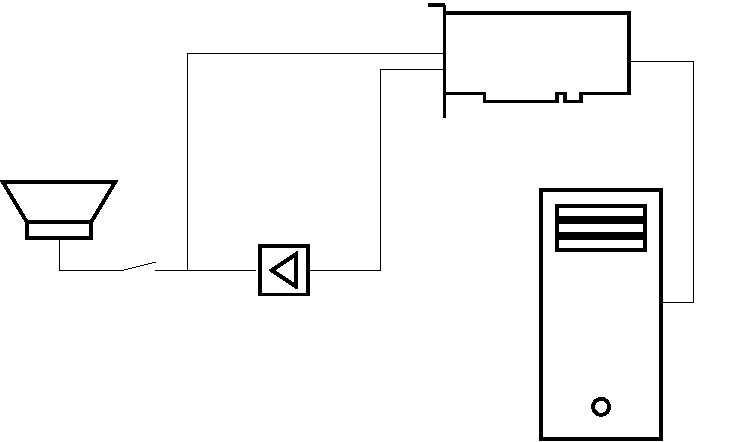
\includegraphics{pioneer_transfer_function.pdf}%
\end{picture}%
\setlength{\unitlength}{2818sp}%
%
\begingroup\makeatletter\ifx\SetFigFont\undefined%
\gdef\SetFigFont#1#2#3#4#5{%
  \reset@font\fontsize{#1}{#2pt}%
  \fontfamily{#3}\fontseries{#4}\fontshape{#5}%
  \selectfont}%
\fi\endgroup%
\begin{picture}(8338,4926)(3838,-7474)
\put(9991,-6361){Computer}%
\put(6661,-6091){Amplifier}%
\put(9271,-3211){Sound Card}%
\put(11746,-4696){USB}%
\put(8236,-3526){Out}%
\put(8281,-3031){In}%
\put(3961,-4336){Loudspeaker}%
\put(5131,-5371){Switch}%
\end{picture}%
\caption{Setup for measuring transfer function}
		\label{fig:appendix:pioneer_response}
\end{figure}

\section*{Test procedure}


\begin{enumerate}
\item The materials are set up as in \autoref{fig:appendix:pioneer_response}.
\item The signal cable is connected between the RME FIREFACE UCX output channel 1 and right Line in on the amplifier.
\item The jack to banana cable is connected between the amplifier right B output channel to the  RME FIREFACE UCX input 1 
\item The input gain of RME FIREFACE UCX at input 1 is set to \SI{20}{\decibel}
\item The input and output channel is specified in the MATLAB function "SynchronizedPlaybackAcquirer" 
\item NOTE! the following two step is preformed in parallel, so the volume nob stays the same for every attenuation. The attenuation is controlled by a volume nob in front of the amplifier.
\item IRmeas_fft (software) \autoref{appendix:transfer_function} is preformed with attenuation of \SI{-40}{\decibel}, \SI{-16}{\decibel}  and  \SI{0}{\decibel} of the amplifier without load 
\item then IRmeas_fft (software) \autoref{appendix:transfer_function} is preformed with attenuation of \SI{-40}{\decibel}, \SI{-16}{\decibel} and \SI{0}{\decibel} of the amplifier with load. 
\item the measurement is done with \texttt{playgain} \SI{-18}{\decibel}, \SI{-42}{\decibel} and \SI{-57}{\decibel} respectively, so the output voltage of the amplifier do not damage the soundcard.
\item The measured transfer function from the RME FIREFACE UCX is subtracted all measurement, to get a true voltage gain of the amplifier.
\item The transfer function is plotted from \SI{20}{\hertz} to \SI{20}{\kilo\hertz} for every measurement, where the measurement with load is plotted first in read, and then the measurement without load is plotted in blue.

\end{enumerate}

\section*{Results}



On \autoref{fig:appendix:amplifier_response_result} it is seen that the transfer function of the amplifier do not depend on an output load, when the load is SEAS 33 F-WKA because the red and blue curve lays up on each other for the three measuring point. The amplifier is not a linear gain factor from \SI{20}{\hertz} to \SI{20}{\kilo\hertz} at high attenuation, because the non linearity at \SI{-40}{\decibel} is \SI{1.75}{\decibel} from the highest to the lowest attenuation. The amplifier get at most a linear gain factor when the attenuation is lowered because the non linearity at an attenuation of \SI{0}{\decibel} is \SI{0.16}{\decibel}. At \SI{-16}{\decibel} the non linearity is \SI{0.55}{\decibel}.



\begin{figure}[H]
	\centering
	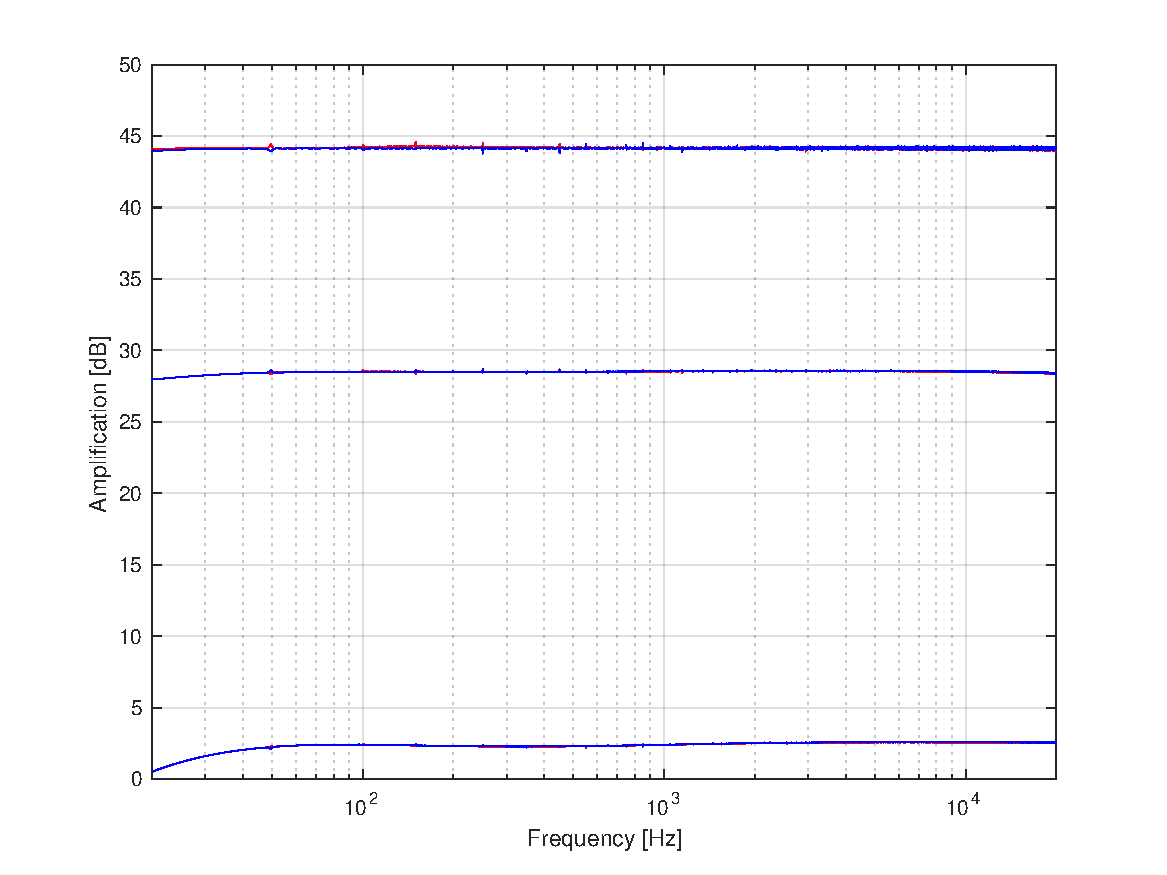
\includegraphics[width=1\textwidth]{transfer_function_of_amplifier.pdf}
	\caption{The frequency response of the Pioneer A-616 there the lower blue and red curve display the attenuation of \SI{-40}{\decibel}. The middle blue and red curve correspond to an attenuation of \SI{-16}{\decibel} and the upper blue and red curve correspond to an attenuation of  \SI{0}{\decibel}}
		\label{fig:appendix:amplifier_response_result}
\end{figure}

\section*{Conclusion}
It can be concluded that the transfer function of the amplifier Pioneer A-616 do not depend on a load on the output. It can also be concluded that the amplifier is a gain factor from \SI{20}{\hertz} to \SI{20}{\kilo\hertz} with attenuation lower than \SI{-16}{\decibel}, because a non linearity of \SI{0.55}{\decibel} or lower is accepted.

